\documentclass[tekniskrapport/tech.tex]{subfiles}

\begin{document}
\section{Produkten}
Taxibilen startas upp genom att först öppna upp det grafiska gränssnittet och
därigenom ansluta den till en dator via en trådlös länk. När bilen väl har en
koppling till datorn är det bara att börja använda den och alla dess
funktioner. Det går att läsa mer om hur den används i taxins användarmanual. I figur
\ref{fig:taxi1} finns en bild över hur taxin ser ut.

\begin{figure}[H]
    \centering
    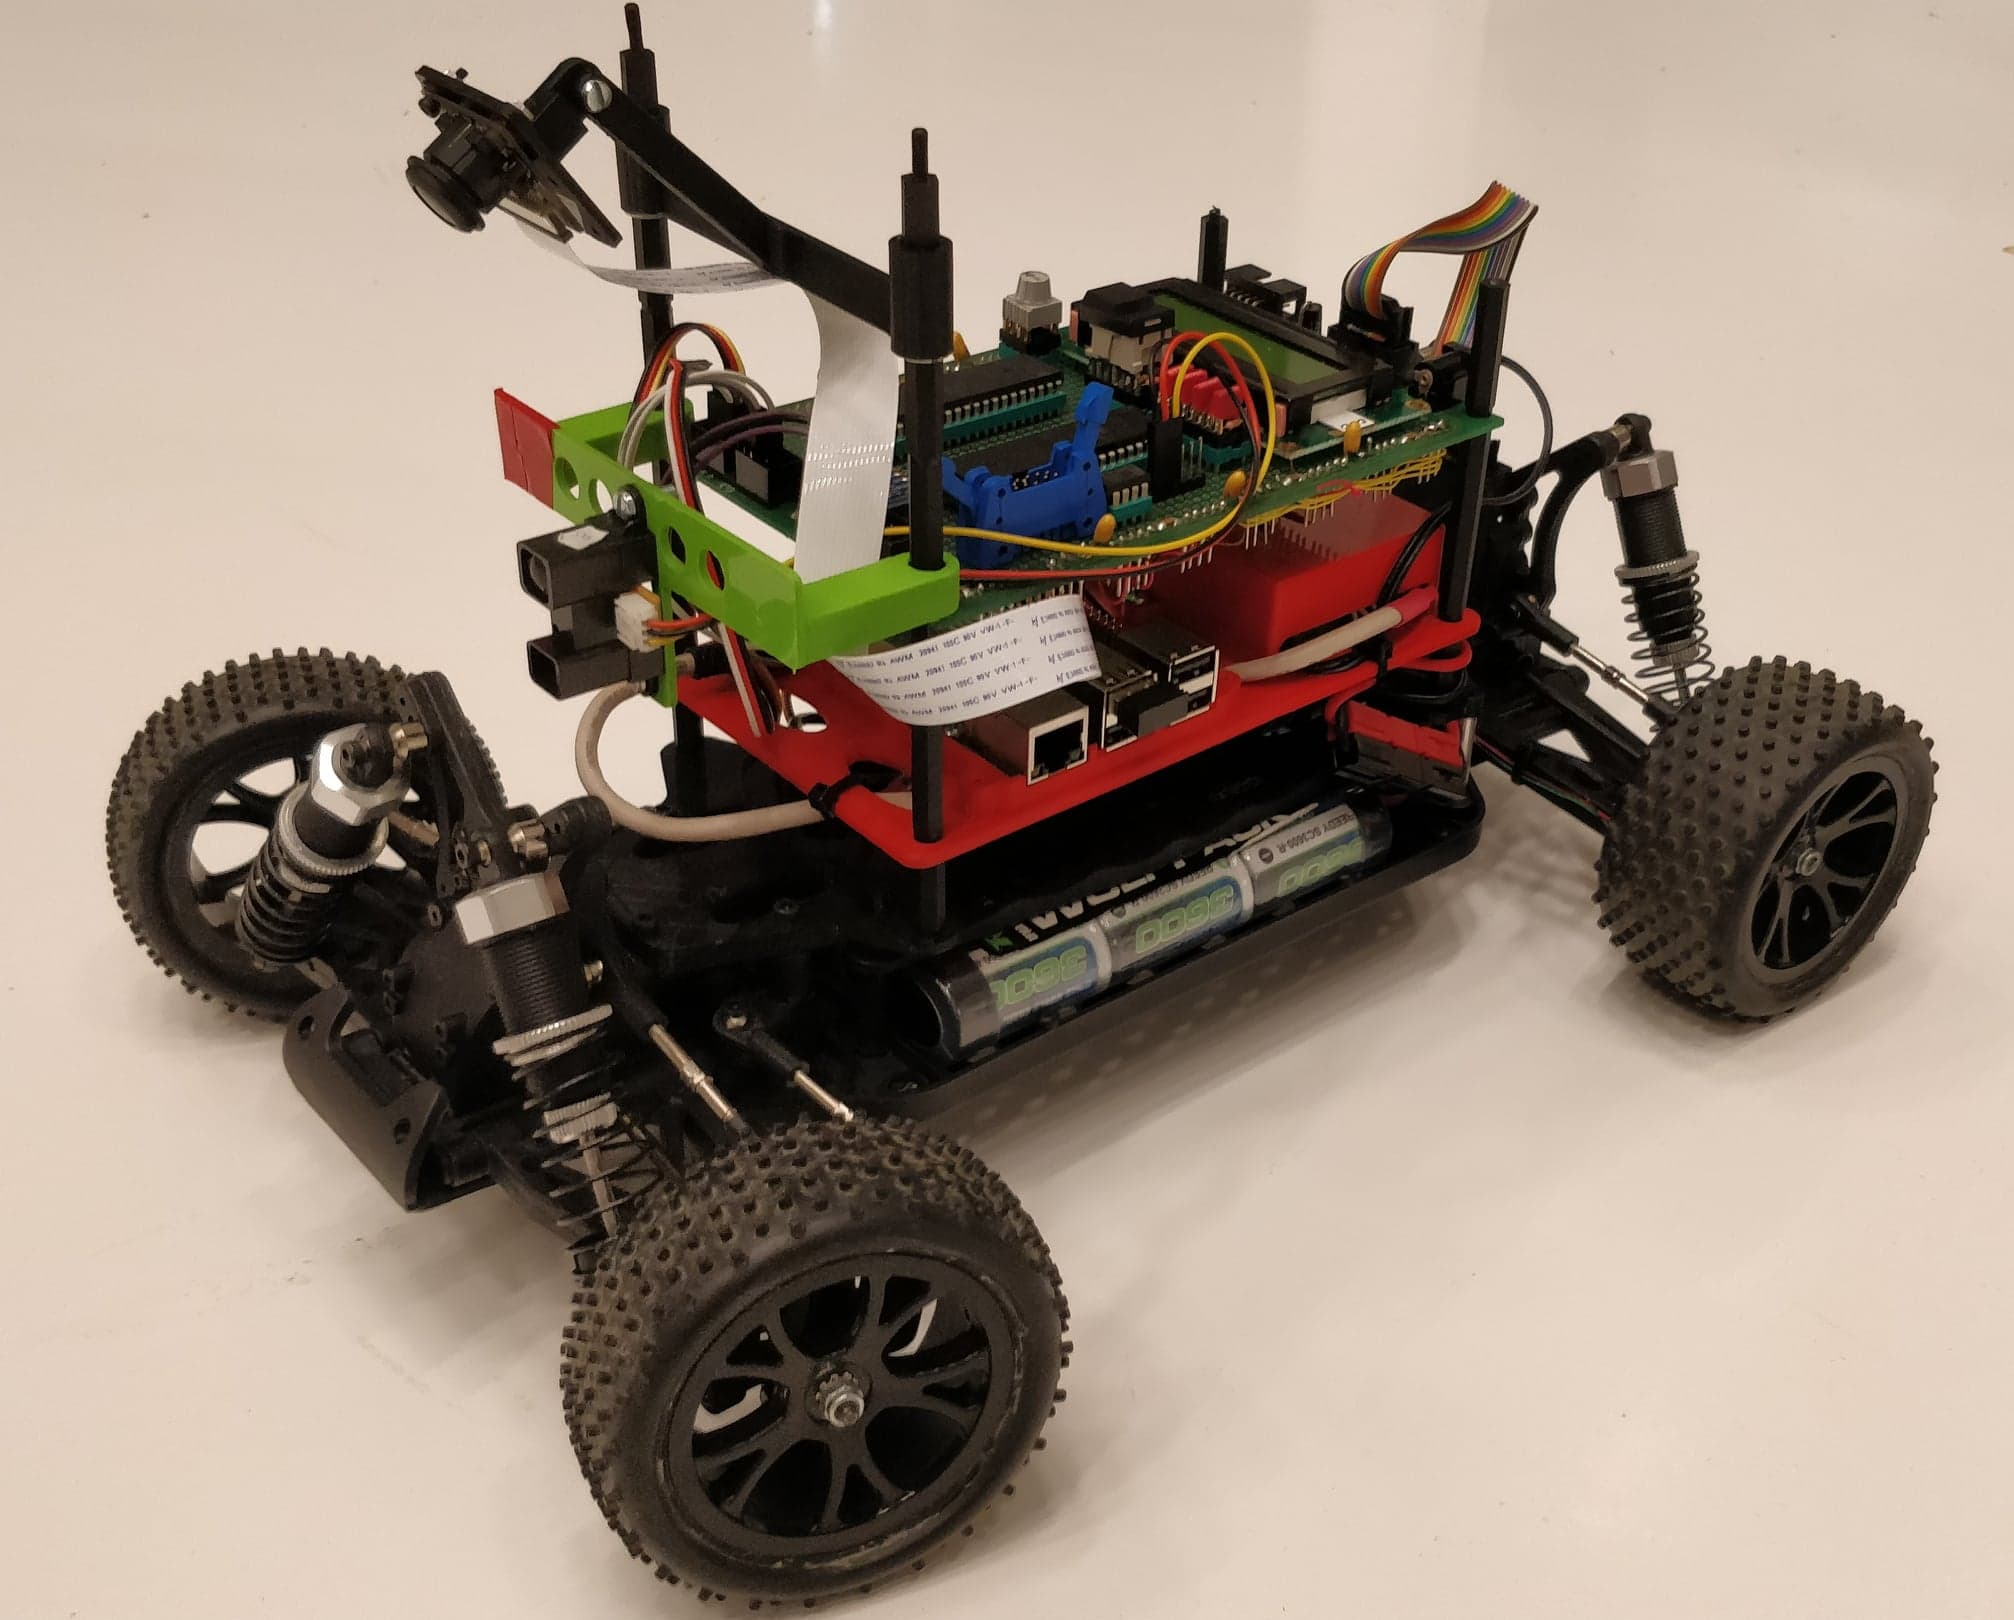
\includegraphics[width=0.8\linewidth]{\figures/taxi1.jpg}
    \caption{Hur den färdiga taxin ser ut.}
    \label{fig:taxi1}
\end{figure}

\noindent
Taxin ska användas till att utföra uppdrag i en speciell bana. Uppdragen går ut
på att hämta upp och släppa av passagerare på olika destinationer i den givna
banan. När taxin väl har startat uppdraget ska den kunna slutföra det helt på
egen hand, alltså autonomt. För att uppdraget ska bli godkänt måste taxin klara
av att navigera banan på ett säkert sätt genom att följa trafikregler och
undvika hinder.
\end{document}
